
\chapter{ಅನುಬಂಧ : II}

\section*{ಬೀಜಗಣಿತದಲ್ಲಿ ಮಾಯಾಚೌಕಗಳ ಬಳಕೆ :}

ಮಾಯಾಚೌಕಗಳನ್ನು ಬೀಜಗಣಿತದ ಕೆಲವು ನಿತ್ಯ ಸಮತೆಗಳನ್ನು (ಐಡೆಂಟಿಟಿ) ಬಿಡಿಸಲು ಬಳಸಬಹುದು. ಶ್ರೀನಿವಾಸ ರಾಮಾನುಜನ್ ಮೊದಲ್ಗೊಂಡು ಕೆಲವು ಗಣಿತ ವಿದ್ವಾಂಸರು ಈ ದಿಕ್ಕಿನಲ್ಲಿ ಸಾಕಷ್ಟು ಕೆಲಸಮಾಡಿದ್ದಾರೆ.

ಒಂದು ಉದಾಹರಣೆ ಮೂಲಕ ಸ್ಪಷ್ಟ ಮಾಡಿಕೊಳ್ಳೋಣ. 3 ಕ್ರಮವರ್ಗದ ಒಂದು ಸರಳ ಮಾಯಾಚೌಕ.
\begin{figure}[H]
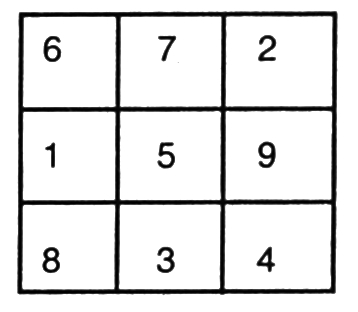
\includegraphics{src/figures/chap10/fig10.1.jpg}
\end{figure}

ಇದರಲ್ಲಿನ ಎಲ್ಲ ಸಂಖ್ಯೆಗಳಿಂದಲೂ 5ನ್ನು ಕಳೆಯೋಣ.
\begin{figure}[H]
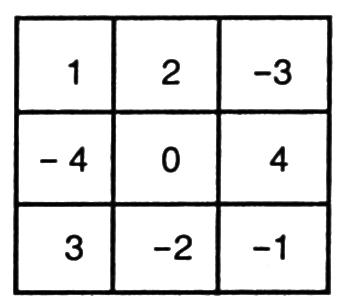
\includegraphics{src/figures/chap10/fig10.2.jpg}
\end{figure}

ಈ ಮಾಯಾಚೌಕದ ಅಡ್ಡಸಾಲು, ಕಂಭಸಾಲು, ಕರ್ಣ ಸಾಲುಗಳ ಮೊತ್ತ 0.

ಇಂತಹ ಮಾಯಾಚೌಕಗಳಿಗೆ ಶೂನ್ಯ ಮಾಯಾಚೌಕ \textbf{(ಜೀರೊ ಮ್ಯಾಜಿಕ್ ಸ್ಕ್ವೇರ್)} ಎಂದು ಹೆಸರಿಸಲಾಗಿದೆ. ಇಂತಹ ಶೂನ್ಯ ಮಾಯಾಚೌಕಗಳ ಸಹಾಯದಿಂದ ಬೀಜಗಣಿತದ ನಿತ್ಯ ಸಮತೆಯನ್ನು ಬಿಡಿಸಬಹುದು.

ಶೂನ್ಯ ಮಾಯಾಚೌಕದಲ್ಲಿನ ಮೊದಲ ಮತ್ತು ಕೊನೆಯ ಅಡ್ಡಸಾಲುಗಳ ಮೊತ್ತವನ್ನು ನೋಡಿ. ಆ ಸಂಖ್ಯೆ-ಗಳ ವರ್-ಗ-ಸಂಖ್ಯೆ-ಗ-ಳನ್ನೂ ಬ-ರೆದು ನೋ-ಡಿ.

$1+2+(-3) =3+(-2)+(-1)$

$12+22+(-3) 2 =32+(-2)^2 +(-1)^2$

ಹಾಗೆಯೇ ಮೊದಲ ಮತ್ತು ಕೊನೆಯ ಕಂಭ ಸಾಲುಗಳ ಮೊತ್ತ ಬರೆಯಿರಿ.

$1+(-4)+3 = -(-3)+4+(-1)$

$1^2+(-4)^2 +3^2 =-(-3)^2+4^2 +(-1)^2$

ಸಂಖ್ಯೆಗಳ ವರ್ಗಗಳನ್ನು ಬರೆದಾಗಲೂ ಸಮೀಕರಣಗಳು ಸಮತ್ವ ತೋರಿಸುತ್ತವೆ.

ಹಾಗಾದರೆ, ಶೂನ್ಯ ಮಾಯಾಚೌಕದ ಎಲ್ಲ ಸಂಖ್ಯೆಗಳಿಗೂ ಯಾವುದಾದರೂ ಒಂದು ಸಂಖ್ಯೆನ್ನು ಕೂಡಿಸಿದರೆ ಬರುವ ಸಮೀಕರಣಗಳು ಸಮತ್ವ ಹೊಂದಿರುತ್ತದೆ.

ವರ್ಗ ಮಾಡಿರುವುದಕ್ಕೆ x ನ್ನು ಸೇರಿಸೋಣ.

$(x+1)^2+(x+2)^2+(x-3)^2 = (x+3)^2+(x-2)^2+(x-1)^2$

ಮತ್ತು $(x+1)^2+(x-4)^2+(x+3)^2 = (x-3)^2+(x+4)^2+(x-1)^2$

ಎರಡೂ ಕಡೆಯ ಪದಗಳನ್ನು ವಿಸ್ತರಿಸಿ, ಸಂಕ್ಷೇಪಿಸಿದರೆ ಈ ಸಮತ್ವ ಸರಿ ಎಂಬುದು ಕಂಡುಬರುತ್ತದೆ.

ಹಾಗಾದರೆ $a^2+b^2+c^2 = p^2+q^2+r^2$ ಇಂತಹ ಎರಡನೆ ಡಿಗ್ರಿಯ ಸಮೀಕರಣವನ್ನು ಮೇಲಿನ ಸಮತ್ವಗಳನ್ನು ಬಳಸಿ ಬಿಡಿಸಬಹುದು ಎಂದಾಯಿತು.
\begin{figure}[H]
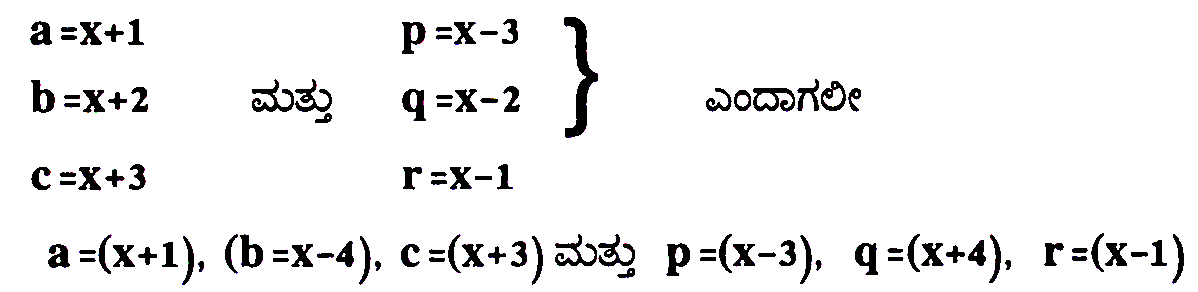
\includegraphics{src/figures/chap10/fig10.3.jpg}
\end{figure}

$a=(x+1), (b=x-4), c=(x+3)$ ಮತ್ತು $p=(x-3), q=(x+4), r=(x-1)$ ಎಂದಾಗಲೀ, ಇಟ್ಟುಗೊಂಡು, a, b, c, p, q, r ಬೆಲೆಗಳನ್ನು ಎರಡನೆಯ ಡಿಗ್ರಿಯ ಸಮೀಕರಣದಲ್ಲಿ ಆದೇಶಿಸಬಹುದು. $x=5$ ಎಂದಿಟ್ಟುಕೊಂಡರೆ.

$a^2 +b^2+c^2= 6^2 + 7^2 + 2^2 = 36 +49 +4=89$

$p^2 q^2 + r^2 = 8^2 3^2 +4^2 = 64 +9 + 16 89$

ಇದರಿಂದ $a^2+b^2+c^2 = p^2+q^2+r^2$ ರೀತಿಯ ನಿತ್ಯ ಸಮತೆ ಐಡೆಂಟಿಟಿಗಳನ್ನು ಬಿಡಿಸಲು ಸಾಧ್ಯ .

$a=6, b-7, c=2, p=8, q=3, r=4$

ಇದೇವಿಧಾನದಲ್ಲಿ $a^2 +b^2 +c^2 d^2 e^2 f^2 = p^2 q^2 r^2 s^2 t^2 u^2$ ನಂತಹ ನಿತ್ಯಸಮತೆಗಳನ್ನು ಬಿಡಿಸಬಹುದು.

(ಹೆಚ್ಚಿನ ವಿವರಗಳನ್ನು ಇಚ್ಛಿಸುವವರು. Harvesting Magic Squares by P.K. Srinivasan, ಪ್ರಕಟಣೆ, allied Publishers ಪುಸ್ತಕವನ್ನು ಪರಾಮರ್ಷಿಸಬಹುದು.)
